% Options for packages loaded elsewhere
\PassOptionsToPackage{unicode}{hyperref}
\PassOptionsToPackage{hyphens}{url}
\PassOptionsToPackage{dvipsnames,svgnames,x11names}{xcolor}
%
\documentclass[
  letterpaper,
  DIV=11,
  numbers=noendperiod]{scrartcl}

\usepackage{amsmath,amssymb}
\usepackage{iftex}
\ifPDFTeX
  \usepackage[T1]{fontenc}
  \usepackage[utf8]{inputenc}
  \usepackage{textcomp} % provide euro and other symbols
\else % if luatex or xetex
  \usepackage{unicode-math}
  \defaultfontfeatures{Scale=MatchLowercase}
  \defaultfontfeatures[\rmfamily]{Ligatures=TeX,Scale=1}
\fi
\usepackage{lmodern}
\ifPDFTeX\else  
    % xetex/luatex font selection
\fi
% Use upquote if available, for straight quotes in verbatim environments
\IfFileExists{upquote.sty}{\usepackage{upquote}}{}
\IfFileExists{microtype.sty}{% use microtype if available
  \usepackage[]{microtype}
  \UseMicrotypeSet[protrusion]{basicmath} % disable protrusion for tt fonts
}{}
\makeatletter
\@ifundefined{KOMAClassName}{% if non-KOMA class
  \IfFileExists{parskip.sty}{%
    \usepackage{parskip}
  }{% else
    \setlength{\parindent}{0pt}
    \setlength{\parskip}{6pt plus 2pt minus 1pt}}
}{% if KOMA class
  \KOMAoptions{parskip=half}}
\makeatother
\usepackage{xcolor}
\setlength{\emergencystretch}{3em} % prevent overfull lines
\setcounter{secnumdepth}{5}
% Make \paragraph and \subparagraph free-standing
\ifx\paragraph\undefined\else
  \let\oldparagraph\paragraph
  \renewcommand{\paragraph}[1]{\oldparagraph{#1}\mbox{}}
\fi
\ifx\subparagraph\undefined\else
  \let\oldsubparagraph\subparagraph
  \renewcommand{\subparagraph}[1]{\oldsubparagraph{#1}\mbox{}}
\fi

\usepackage{color}
\usepackage{fancyvrb}
\newcommand{\VerbBar}{|}
\newcommand{\VERB}{\Verb[commandchars=\\\{\}]}
\DefineVerbatimEnvironment{Highlighting}{Verbatim}{commandchars=\\\{\}}
% Add ',fontsize=\small' for more characters per line
\usepackage{framed}
\definecolor{shadecolor}{RGB}{241,243,245}
\newenvironment{Shaded}{\begin{snugshade}}{\end{snugshade}}
\newcommand{\AlertTok}[1]{\textcolor[rgb]{0.68,0.00,0.00}{#1}}
\newcommand{\AnnotationTok}[1]{\textcolor[rgb]{0.37,0.37,0.37}{#1}}
\newcommand{\AttributeTok}[1]{\textcolor[rgb]{0.40,0.45,0.13}{#1}}
\newcommand{\BaseNTok}[1]{\textcolor[rgb]{0.68,0.00,0.00}{#1}}
\newcommand{\BuiltInTok}[1]{\textcolor[rgb]{0.00,0.23,0.31}{#1}}
\newcommand{\CharTok}[1]{\textcolor[rgb]{0.13,0.47,0.30}{#1}}
\newcommand{\CommentTok}[1]{\textcolor[rgb]{0.37,0.37,0.37}{#1}}
\newcommand{\CommentVarTok}[1]{\textcolor[rgb]{0.37,0.37,0.37}{\textit{#1}}}
\newcommand{\ConstantTok}[1]{\textcolor[rgb]{0.56,0.35,0.01}{#1}}
\newcommand{\ControlFlowTok}[1]{\textcolor[rgb]{0.00,0.23,0.31}{#1}}
\newcommand{\DataTypeTok}[1]{\textcolor[rgb]{0.68,0.00,0.00}{#1}}
\newcommand{\DecValTok}[1]{\textcolor[rgb]{0.68,0.00,0.00}{#1}}
\newcommand{\DocumentationTok}[1]{\textcolor[rgb]{0.37,0.37,0.37}{\textit{#1}}}
\newcommand{\ErrorTok}[1]{\textcolor[rgb]{0.68,0.00,0.00}{#1}}
\newcommand{\ExtensionTok}[1]{\textcolor[rgb]{0.00,0.23,0.31}{#1}}
\newcommand{\FloatTok}[1]{\textcolor[rgb]{0.68,0.00,0.00}{#1}}
\newcommand{\FunctionTok}[1]{\textcolor[rgb]{0.28,0.35,0.67}{#1}}
\newcommand{\ImportTok}[1]{\textcolor[rgb]{0.00,0.46,0.62}{#1}}
\newcommand{\InformationTok}[1]{\textcolor[rgb]{0.37,0.37,0.37}{#1}}
\newcommand{\KeywordTok}[1]{\textcolor[rgb]{0.00,0.23,0.31}{#1}}
\newcommand{\NormalTok}[1]{\textcolor[rgb]{0.00,0.23,0.31}{#1}}
\newcommand{\OperatorTok}[1]{\textcolor[rgb]{0.37,0.37,0.37}{#1}}
\newcommand{\OtherTok}[1]{\textcolor[rgb]{0.00,0.23,0.31}{#1}}
\newcommand{\PreprocessorTok}[1]{\textcolor[rgb]{0.68,0.00,0.00}{#1}}
\newcommand{\RegionMarkerTok}[1]{\textcolor[rgb]{0.00,0.23,0.31}{#1}}
\newcommand{\SpecialCharTok}[1]{\textcolor[rgb]{0.37,0.37,0.37}{#1}}
\newcommand{\SpecialStringTok}[1]{\textcolor[rgb]{0.13,0.47,0.30}{#1}}
\newcommand{\StringTok}[1]{\textcolor[rgb]{0.13,0.47,0.30}{#1}}
\newcommand{\VariableTok}[1]{\textcolor[rgb]{0.07,0.07,0.07}{#1}}
\newcommand{\VerbatimStringTok}[1]{\textcolor[rgb]{0.13,0.47,0.30}{#1}}
\newcommand{\WarningTok}[1]{\textcolor[rgb]{0.37,0.37,0.37}{\textit{#1}}}

\providecommand{\tightlist}{%
  \setlength{\itemsep}{0pt}\setlength{\parskip}{0pt}}\usepackage{longtable,booktabs,array}
\usepackage{calc} % for calculating minipage widths
% Correct order of tables after \paragraph or \subparagraph
\usepackage{etoolbox}
\makeatletter
\patchcmd\longtable{\par}{\if@noskipsec\mbox{}\fi\par}{}{}
\makeatother
% Allow footnotes in longtable head/foot
\IfFileExists{footnotehyper.sty}{\usepackage{footnotehyper}}{\usepackage{footnote}}
\makesavenoteenv{longtable}
\usepackage{graphicx}
\makeatletter
\def\maxwidth{\ifdim\Gin@nat@width>\linewidth\linewidth\else\Gin@nat@width\fi}
\def\maxheight{\ifdim\Gin@nat@height>\textheight\textheight\else\Gin@nat@height\fi}
\makeatother
% Scale images if necessary, so that they will not overflow the page
% margins by default, and it is still possible to overwrite the defaults
% using explicit options in \includegraphics[width, height, ...]{}
\setkeys{Gin}{width=\maxwidth,height=\maxheight,keepaspectratio}
% Set default figure placement to htbp
\makeatletter
\def\fps@figure{htbp}
\makeatother
% definitions for citeproc citations
\NewDocumentCommand\citeproctext{}{}
\NewDocumentCommand\citeproc{mm}{%
  \begingroup\def\citeproctext{#2}\cite{#1}\endgroup}
\makeatletter
 % allow citations to break across lines
 \let\@cite@ofmt\@firstofone
 % avoid brackets around text for \cite:
 \def\@biblabel#1{}
 \def\@cite#1#2{{#1\if@tempswa , #2\fi}}
\makeatother
\newlength{\cslhangindent}
\setlength{\cslhangindent}{1.5em}
\newlength{\csllabelwidth}
\setlength{\csllabelwidth}{3em}
\newenvironment{CSLReferences}[2] % #1 hanging-indent, #2 entry-spacing
 {\begin{list}{}{%
  \setlength{\itemindent}{0pt}
  \setlength{\leftmargin}{0pt}
  \setlength{\parsep}{0pt}
  % turn on hanging indent if param 1 is 1
  \ifodd #1
   \setlength{\leftmargin}{\cslhangindent}
   \setlength{\itemindent}{-1\cslhangindent}
  \fi
  % set entry spacing
  \setlength{\itemsep}{#2\baselineskip}}}
 {\end{list}}
\usepackage{calc}
\newcommand{\CSLBlock}[1]{\hfill\break\parbox[t]{\linewidth}{\strut\ignorespaces#1\strut}}
\newcommand{\CSLLeftMargin}[1]{\parbox[t]{\csllabelwidth}{\strut#1\strut}}
\newcommand{\CSLRightInline}[1]{\parbox[t]{\linewidth - \csllabelwidth}{\strut#1\strut}}
\newcommand{\CSLIndent}[1]{\hspace{\cslhangindent}#1}

% load packages
\usepackage{geometry}
\usepackage{xcolor}
\usepackage{eso-pic}
\usepackage{fancyhdr}
\usepackage{sectsty}
\usepackage{fontspec}
\usepackage{titlesec}

%% Set page size with a wider right margin
\geometry{a4paper, total={170mm,257mm}, left=20mm, top=20mm, bottom=20mm, right=50mm}

%% Let's define some colours
\definecolor{uniblue}{HTML}{003865}
\definecolor{burgundy}{HTML}{7D2239}
\definecolor{cobalt}{HTML}{005C8A}
\definecolor{lavender}{HTML}{5B4D94}
\definecolor{leaf}{HTML}{006630}
\definecolor{moss}{HTML}{385A4F}
\definecolor{pillarbox}{HTML}{B30C00}
\definecolor{rust}{HTML}{9A3A06}
\definecolor{sandstone}{HTML}{52473B}
\definecolor{skyblue}{HTML}{005398}
\definecolor{slate}{HTML}{4F5961}
\definecolor{thistle}{HTML}{951272}

%\definecolor{light}{HTML}{E6E6FA} % original from template - redefined below as uni blue at 10 percent:
\colorlet{light}{uniblue!10}
%\definecolor{highlight}{HTML}{800080} % original from template - redefined below as uni's skyblue:
\colorlet{highlight}{skyblue}
%\definecolor{dark}{HTML}{330033} % original from template - redefined below as uni blue at 100 percent:
\colorlet{dark}{uniblue}

%% Let's add the border on the right hand side 
\AddToShipoutPicture{% 
    \AtPageLowerLeft{% 
        \put(\LenToUnit{\dimexpr\paperwidth-3cm},0){% 
            \color{light}\rule{3cm}{\LenToUnit\paperheight}%
          }%
     }%
     % logo
    \AtPageLowerLeft{% start the bar at the bottom right of the page
        \put(\LenToUnit{\dimexpr\paperwidth-2.25cm},27.2cm){% move it to the top right
            \color{light}
\includegraphics[width=2.25cm]{_extensions/nrennie/PrettyPDF/uni_logo_boxed.jpg}
          }%
     }%
}

%% Style the page number
\fancypagestyle{mystyle}{
  \fancyhf{}
  \renewcommand\headrulewidth{0pt}
  \fancyfoot[R]{\thepage}
  \fancyfootoffset{3.5cm}
}
\setlength{\footskip}{20pt}

%% style the chapter/section fonts
\chapterfont{\color{uniblue}\fontsize{20}{16.8}\selectfont}
\sectionfont{\color{uniblue}\fontsize{20}{16.8}\selectfont}
\subsectionfont{\color{skyblue}\fontsize{14}{16.8}\selectfont}
\titleformat{\subsection}
  {\color{uniblue!90}\sffamily\Large\bfseries}{\thesubsection}{1em}{}[{\titlerule[0.8pt]}]
\subsubsectionfont{\color{cobalt}}

\renewcommand\thesection{\color{slate}\arabic{section}}
  
% left align title
\makeatletter
\renewcommand{\maketitle}{\bgroup\setlength{\parindent}{0pt}
\begin{flushleft}
  {\color{uniblue}\sffamily\huge\textbf{\@title}} \vspace{0.3cm} \newline
  {\Large {\@subtitle}} \newline
  \@author
\end{flushleft}\egroup
}
\makeatother

%% Use some custom fonts
\setsansfont{Ubuntu}[
    Path=_extensions/nrennie/PrettyPDF/Ubuntu/,
    Scale=0.9,
    Extension = .ttf,
    UprightFont=*-Regular,
    BoldFont=*-Bold,
    ItalicFont=*-Italic,
    ]

\setmainfont{Ubuntu}[
    Path=_extensions/nrennie/PrettyPDF/Ubuntu/,
    Scale=0.9,
    Extension = .ttf,
    UprightFont=*-Regular,
    BoldFont=*-Bold,
    ItalicFont=*-Italic,
    ]
\usepackage{cancel}
\KOMAoption{captions}{tableheading}
\makeatletter
\@ifpackageloaded{tcolorbox}{}{\usepackage[skins,breakable]{tcolorbox}}
\@ifpackageloaded{fontawesome5}{}{\usepackage{fontawesome5}}
\definecolor{quarto-callout-color}{HTML}{909090}
\definecolor{quarto-callout-note-color}{HTML}{0758E5}
\definecolor{quarto-callout-important-color}{HTML}{CC1914}
\definecolor{quarto-callout-warning-color}{HTML}{EB9113}
\definecolor{quarto-callout-tip-color}{HTML}{00A047}
\definecolor{quarto-callout-caution-color}{HTML}{FC5300}
\definecolor{quarto-callout-color-frame}{HTML}{acacac}
\definecolor{quarto-callout-note-color-frame}{HTML}{4582ec}
\definecolor{quarto-callout-important-color-frame}{HTML}{d9534f}
\definecolor{quarto-callout-warning-color-frame}{HTML}{f0ad4e}
\definecolor{quarto-callout-tip-color-frame}{HTML}{02b875}
\definecolor{quarto-callout-caution-color-frame}{HTML}{fd7e14}
\makeatother
\makeatletter
\@ifpackageloaded{caption}{}{\usepackage{caption}}
\AtBeginDocument{%
\ifdefined\contentsname
  \renewcommand*\contentsname{Table of contents}
\else
  \newcommand\contentsname{Table of contents}
\fi
\ifdefined\listfigurename
  \renewcommand*\listfigurename{List of Figures}
\else
  \newcommand\listfigurename{List of Figures}
\fi
\ifdefined\listtablename
  \renewcommand*\listtablename{List of Tables}
\else
  \newcommand\listtablename{List of Tables}
\fi
\ifdefined\figurename
  \renewcommand*\figurename{Figure}
\else
  \newcommand\figurename{Figure}
\fi
\ifdefined\tablename
  \renewcommand*\tablename{Table}
\else
  \newcommand\tablename{Table}
\fi
}
\@ifpackageloaded{float}{}{\usepackage{float}}
\floatstyle{ruled}
\@ifundefined{c@chapter}{\newfloat{codelisting}{h}{lop}}{\newfloat{codelisting}{h}{lop}[chapter]}
\floatname{codelisting}{Listing}
\newcommand*\listoflistings{\listof{codelisting}{List of Listings}}
\makeatother
\makeatletter
\makeatother
\makeatletter
\@ifpackageloaded{caption}{}{\usepackage{caption}}
\@ifpackageloaded{subcaption}{}{\usepackage{subcaption}}
\makeatother
\makeatletter
\@ifpackageloaded{tcolorbox}{}{\usepackage[skins,breakable]{tcolorbox}}
\makeatother
\makeatletter
\@ifundefined{shadecolor}{\definecolor{shadecolor}{rgb}{.97, .97, .97}}{}
\makeatother
\makeatletter
\@ifundefined{codebgcolor}{\definecolor{codebgcolor}{named}{light}}{}
\makeatother
\makeatletter
\ifdefined\Shaded\renewenvironment{Shaded}{\begin{tcolorbox}[breakable, enhanced, colback={codebgcolor}, sharp corners, boxrule=0pt, frame hidden]}{\end{tcolorbox}}\fi
\makeatother
\ifLuaTeX
  \usepackage{selnolig}  % disable illegal ligatures
\fi
\usepackage{bookmark}

\IfFileExists{xurl.sty}{\usepackage{xurl}}{} % add URL line breaks if available
\urlstyle{same} % disable monospaced font for URLs
\hypersetup{
  pdftitle={Generalised Linear Models part 2},
  colorlinks=true,
  linkcolor={highlight},
  filecolor={Maroon},
  citecolor={Blue},
  urlcolor={highlight},
  pdfcreator={LaTeX via pandoc}}

\title{Generalised Linear Models part 2}
\author{}
\date{}

\begin{document}
\maketitle

\pagestyle{mystyle}

\section{Introduction}\label{introduction}

Last week we introduced \textbf{Generalised Linear Models} (GLMs).
Particularly, we looked at \textbf{logistic regression} to model
outcomes of interest that take one of two categorical values
(e.g.yes/no, success/failure, alive/dead). This week we will continue
reviewing logistic regression to model grouped binary outcomes
(e.g.~number of successes out of a fixed number of trials) and then we
we will generalise this to situations where the response variable is
categorical with more than two categories. First lets look at the
framework for modelling categorical data with only two categories, i.e.

\begin{itemize}
\item
  \textbf{binary}, taking the value 1 (say success, with probability
  \(p\)) or 0 (failure, with probability \(1-p\)) or
\item
  \textbf{binomial}, where \(y_i\) is the number of events (successes)
  in a given number of trials \(n_i\), with the probability of success
  being \(p_i\) and the probability of failure being \(1-p_i\).
\end{itemize}

In both cases the distribution of \(y_i\) is assumed to be binomial, but
in the first case it is \(\mathrm{Bin}(1,p_i)\) and in the second case
it is \(\mathrm{Bin}(n_i,p_i)\). The first case was covered last week,
so now lets focus on the second case.

Before we proceed, we will load all the packages needed for this week:

\begin{Shaded}
\begin{Highlighting}[]
\FunctionTok{library}\NormalTok{(tidyverse)}
\FunctionTok{library}\NormalTok{(ggplot2)}
\FunctionTok{library}\NormalTok{(sjPlot)}
\FunctionTok{library}\NormalTok{(broom)}
\FunctionTok{library}\NormalTok{(performance)}
\FunctionTok{library}\NormalTok{(yardstick)}
\end{Highlighting}
\end{Shaded}

\section{Logistic regression with grouped binary
data}\label{logistic-regression-with-grouped-binary-data}

Suppose that our binary outcome \(y_i\) is grouped across \(n_i\) number
of trials, e.g.~number of times a head landed when a coin was tossed on
multiple occasions or the proportion of beetles that were killed after
being exposed to an insecticide.

In such cases \(y_i \sim \mathrm{Bin}(n_i,p_i)\), often referred to as
proportional data, since our dependent variables are expressed as
percentages or fractions of a whole. Lets look at a an example.

It is known that the incubation temperature can affect the sex
determination of turtles. An experiment was conducted where turtle eggs
were incubated at various temperatures and the number of male and female
hatchlings was recorded. The goal of the experiment was to examine the
link between incubation temperature and the chance of hatchling being a
male.

\begin{center}
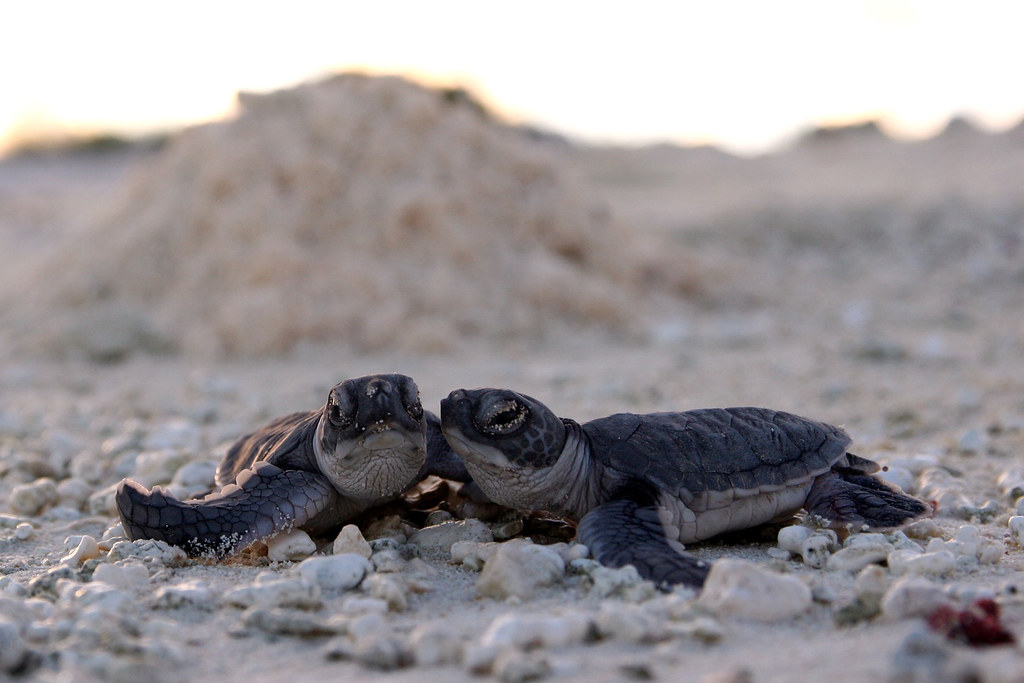
\includegraphics[width=4.92708in,height=\textheight]{turtles.jpg}
\end{center}

The \texttt{turtle} data set contains the number of hatched male and
female turtles across different temperatures, with 3 independent
replicates for each temperature.

The data can be downloaded below:

You can download today's session R script below:

\begin{Shaded}
\begin{Highlighting}[]
\NormalTok{turtles }\OtherTok{=} \FunctionTok{read.csv}\NormalTok{(}\StringTok{"turtles.csv"}\NormalTok{)}
\NormalTok{turtles}\SpecialCharTok{\%\textgreater{}\%} \FunctionTok{glimpse}\NormalTok{()}
\end{Highlighting}
\end{Shaded}

\begin{verbatim}
Rows: 15
Columns: 3
$ temp   <dbl> 27.2, 27.2, 27.2, 27.7, 27.7, 27.7, 28.3, 28.3, 28.3, 28.4, 28.~
$ male   <int> 1, 0, 1, 7, 4, 6, 13, 6, 7, 7, 5, 7, 10, 8, 9
$ female <int> 9, 8, 8, 3, 2, 2, 0, 3, 1, 3, 3, 2, 1, 0, 0
\end{verbatim}

Lets investigate whether the probability of a male being hatched
increases or decrease with the temperature. First, we need to compute
the proportion of males that hatched on each replicate per temperature.
To do this, we obtain the ratio between the total number of male
hatchlings and total number hatchlings (males+females):

\begin{Shaded}
\begin{Highlighting}[]
\NormalTok{turtles }\OtherTok{=}\NormalTok{ turtles }\SpecialCharTok{\%\textgreater{}\%} 
  \FunctionTok{mutate}\NormalTok{(}\AttributeTok{totals =}\NormalTok{ male}\SpecialCharTok{+}\NormalTok{female,}
         \AttributeTok{male\_props =}\NormalTok{ male}\SpecialCharTok{/}\NormalTok{totals)}
\end{Highlighting}
\end{Shaded}

We can see on the next plot, that the proportion of males hatchlings
seems to increase as the incubation temperature rises.

\begin{Shaded}
\begin{Highlighting}[]
\FunctionTok{ggplot}\NormalTok{(turtles,}\FunctionTok{aes}\NormalTok{(}\AttributeTok{y=}\NormalTok{ male\_props,}\AttributeTok{x=}\NormalTok{temp))}\SpecialCharTok{+}
  \FunctionTok{geom\_point}\NormalTok{()}\SpecialCharTok{+} 
  \FunctionTok{labs}\NormalTok{(}\AttributeTok{y=}\StringTok{"proportion of male hatchlings"}\NormalTok{,}\AttributeTok{x =} \StringTok{"temperature"}\NormalTok{)}
\end{Highlighting}
\end{Shaded}

\begin{center}
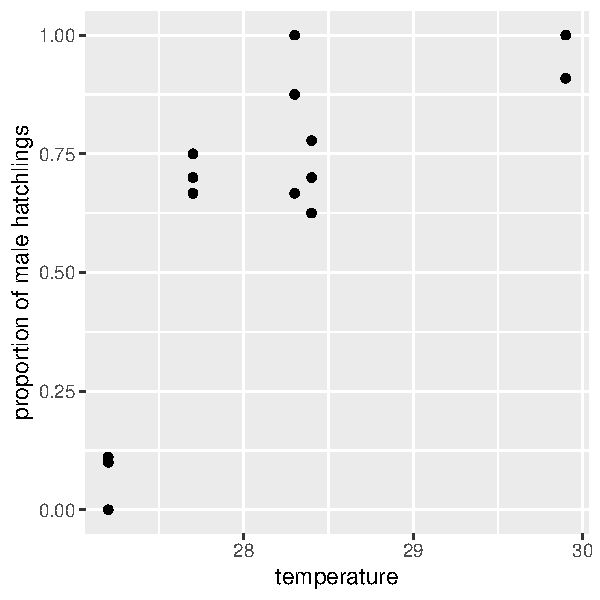
\includegraphics{index_files/figure-pdf/unnamed-chunk-5-1.pdf}
\end{center}

To corroborate this result, we can fit a logistic regression to the
data.

\begin{align}
y_i &\sim \mathrm{Binomial}(n_i,p_i)\\
\mathrm{logit}(p_i) &= \beta_0 +\beta_1 \times \mathrm{temperature}.
\end{align}

Here, \(y_i\) denotes the number of hatched males on the \(i\)th
experiment replicate, \(n_i\) is the fixed total number of hatched eggs
per replicate, \(p_i\) is the probability of a male turtle being
hatched, and \(\beta_0\) and \(\beta_1\) are our unknown parameters to
be estimated.

Proportions can be modelled by providing an \(N \times 2\) matrix of the
number of positive events (num. of males hatchlings) and the number of
negative events (number of female hatchlings):

\begin{Shaded}
\begin{Highlighting}[]
\NormalTok{model\_turtles }\OtherTok{\textless{}{-}} \FunctionTok{glm}\NormalTok{(}\FunctionTok{cbind}\NormalTok{(male,female) }\SpecialCharTok{\textasciitilde{}}\NormalTok{ temp,}
                     \AttributeTok{data =}\NormalTok{ turtles,}
                     \AttributeTok{family =}\NormalTok{ binomial)}
\end{Highlighting}
\end{Shaded}

or by providing the proportion of males hatchlings and \texttt{weights}
totals, i.e the number of trials (number of eggs in each replicate), in
the \texttt{glm} function:

\begin{Shaded}
\begin{Highlighting}[]
\NormalTok{model\_turtles }\OtherTok{\textless{}{-}} \FunctionTok{glm}\NormalTok{(male\_props }\SpecialCharTok{\textasciitilde{}}\NormalTok{ temp,}
                     \AttributeTok{data =}\NormalTok{ turtles,}
                     \AttributeTok{weights =}\NormalTok{  totals,}
                     \AttributeTok{family =}\NormalTok{ binomial)}
\end{Highlighting}
\end{Shaded}

These two formulations are valid and will yield to the same following
result:

\begin{Shaded}
\begin{Highlighting}[]
\NormalTok{model\_turtles }\SpecialCharTok{\%\textgreater{}\%} \FunctionTok{tab\_model}\NormalTok{(}\AttributeTok{transform =} \ConstantTok{NULL}\NormalTok{)}
\end{Highlighting}
\end{Shaded}

\begin{longtable}[]{@{}cccc@{}}
\toprule\noalign{}
\endhead
\bottomrule\noalign{}
\endlastfoot
~ & \multicolumn{3}{c@{}}{%
male props} \\
Predictors & Log-Odds & CI & p \\
(Intercept) & -61.32 & -86.83~--~-39.73 & \textbf{\textless0.001} \\
temp & 2.21 & 1.44~--~3.13 & \textbf{\textless0.001} \\
Observations & \multicolumn{3}{l@{}}{%
15} \\
\end{longtable}

Recall that by setting \texttt{transform\ =\ NULL} we get the log-oddss
estimates. Thus, the interpretation goes as follows:

\begin{itemize}
\item
  For every unit increase (celsius degrees presumably) in
  \emph{Temperature,} the log-odds of a male being hatched increase by
  2.21 i.e.~the chances of hatching a male increases as the incubation
  temperature increases.
\item
  Given \(p_{val} < 0.05\), we can \textbf{reject the null hypothesis}
  \(\beta_1 = 0\) that one unit increase in temperature does not affect
  chances of a male being hatched.
\item
  For every unit increase in \emph{Temperature}, the \textbf{odds} of
  hatching a male are \(\mathrm{exp}(\beta_1) = 9.13\) times the odds of
  those with one \emph{temperature} unit less.
\end{itemize}

\begin{tcolorbox}[enhanced jigsaw, leftrule=.75mm, arc=.35mm, colback=white, opacityback=0, breakable, title={Question}, toprule=.15mm, opacitybacktitle=0.6, titlerule=0mm, rightrule=.15mm, bottomtitle=1mm, coltitle=black, toptitle=1mm, colframe=quarto-callout-tip-color-frame, bottomrule=.15mm, colbacktitle=quarto-callout-tip-color!10!white, left=2mm]

If an egg is incubated at a temperature of 27.5 degrees, what are the
odds of a \textbf{female} being hatched?

I need a hint

Firs we can compute:

\begin{enumerate}
\def\labelenumi{\arabic{enumi}.}
\item
  \(\text{Odds(male|temp=27.5)} = \exp(\hat{\beta_0} +\hat{\beta_1} \times 27.5) \approx 0.59\).

  However, we are interested in \(\text{Odds(female|temp=27.5)}\), thus
\item
  \(\text{Odds(female|temp=27.5)}~ = \mathrm{exp}\left(-\left[\hat{\beta_0} +\hat{\beta_1} \times 27.5\right]\right) \approx 1.67\).
\end{enumerate}

\begin{itemize}
\tightlist
\item
  \begin{enumerate}
  \def\labelenumi{(\Alph{enumi})}
  \tightlist
  \item
    The chances of an male being hatched are 59\% greater than a female
    hatchling if the egg was incubated at a temperature of 27.5
    degrees\\
  \end{enumerate}
\item
  \begin{enumerate}
  \def\labelenumi{(\Alph{enumi})}
  \setcounter{enumi}{1}
  \tightlist
  \item
    The chances of an female being hatched are 59\% greater than a male
    hatchling if the egg was incubated at a temperature of 27.5
    degrees\\
  \end{enumerate}
\item
  \begin{enumerate}
  \def\labelenumi{(\Alph{enumi})}
  \setcounter{enumi}{2}
  \tightlist
  \item
    The chances of an female being hatched are approximately 67\%
    greater than a male hatchling if the egg was incubated at a
    temperature of 27.5 degrees\\
  \end{enumerate}
\item
  \begin{enumerate}
  \def\labelenumi{(\Alph{enumi})}
  \setcounter{enumi}{3}
  \tightlist
  \item
    The chances of an male being hatched are 67 greater than a female
    hatchling if the egg was incubated at a temperature of 27.5 degrees
  \end{enumerate}
\end{itemize}

\end{tcolorbox}

We can now plot the predicted probabilities of a hatchling being male.
However, notice that the number of unique temperature values in the
\texttt{turtles} data set is not very large:

\begin{Shaded}
\begin{Highlighting}[]
\NormalTok{ turtles }\SpecialCharTok{\%\textgreater{}\%} \FunctionTok{select}\NormalTok{(temp) }\SpecialCharTok{\%\textgreater{}\%} \FunctionTok{unique}\NormalTok{() }
\end{Highlighting}
\end{Shaded}

\begin{verbatim}
   temp
1  27.2
4  27.7
7  28.3
10 28.4
13 29.9
\end{verbatim}

Thus, we can create a coarser grid of temperature values to make our
predictions and then use the \texttt{plot\_model()} function as follows:

\begin{Shaded}
\begin{Highlighting}[]
\NormalTok{temp\_pred }\OtherTok{=} \FunctionTok{seq}\NormalTok{(}\DecValTok{27}\NormalTok{,}\DecValTok{30}\NormalTok{,}\AttributeTok{by=}\FloatTok{0.01}\NormalTok{)}
\FunctionTok{plot\_model}\NormalTok{(model\_turtles, }
           \AttributeTok{type =} \StringTok{"eff"}\NormalTok{, }
           \AttributeTok{title =} \StringTok{""}\NormalTok{, }
           \AttributeTok{terms=}\StringTok{"temp[temp\_pred]"}\NormalTok{, }
           \AttributeTok{axis.title =} \FunctionTok{c}\NormalTok{(}\StringTok{"Temperature"}\NormalTok{, }\StringTok{"Prob. of a hatchling being male"}\NormalTok{))}
\end{Highlighting}
\end{Shaded}

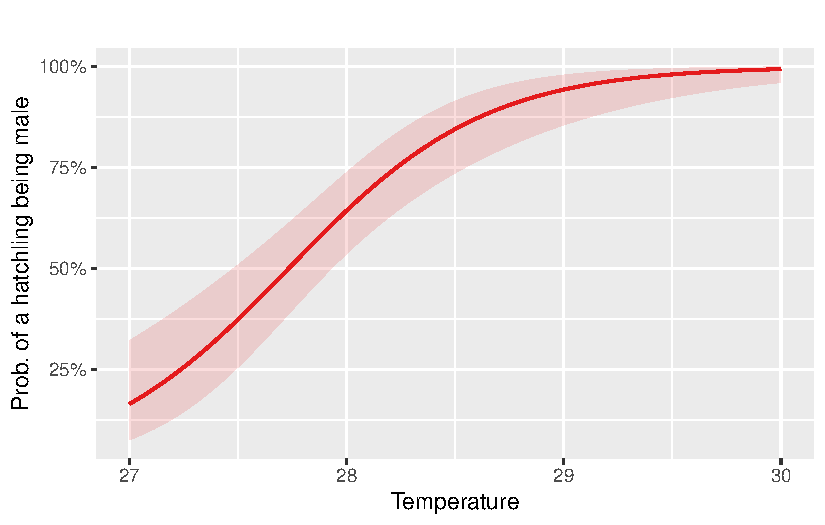
\includegraphics{index_files/figure-pdf/unnamed-chunk-11-1.pdf}

\begin{tcolorbox}[enhanced jigsaw, leftrule=.75mm, arc=.35mm, colback=white, opacityback=0, breakable, title={Question}, toprule=.15mm, opacitybacktitle=0.6, titlerule=0mm, rightrule=.15mm, bottomtitle=1mm, coltitle=black, toptitle=1mm, colframe=quarto-callout-tip-color-frame, bottomrule=.15mm, colbacktitle=quarto-callout-tip-color!10!white, left=2mm]

What is the probability of a turtle egg that is incubated in a
temperature of 28.5 degrees to become a male?

I need a hint

Recall that
\(P~ (male) = \dfrac{Odds(male)}{1 + Odds(male)} = \dfrac{\mathrm{exp}(\hat{\beta_0} +\hat{\beta_1} \times temperature)}{1 + \mathrm{exp}(\hat{\beta_0} +\hat{\beta_1} \times temperature)}\).
In R, the inverse logit transformation can be achieved using the
\texttt{plogis()} function directly on the log-odds. i.e.,
\texttt{plogis(x)=\ exp(x)/1+exp(x)}

\begin{itemize}
\tightlist
\item
  \begin{enumerate}
  \def\labelenumi{(\Alph{enumi})}
  \tightlist
  \item
    0.45\\
  \end{enumerate}
\item
  \begin{enumerate}
  \def\labelenumi{(\Alph{enumi})}
  \setcounter{enumi}{1}
  \tightlist
  \item
    0.18\\
  \end{enumerate}
\item
  \begin{enumerate}
  \def\labelenumi{(\Alph{enumi})}
  \setcounter{enumi}{2}
  \tightlist
  \item
    0.84\\
  \end{enumerate}
\item
  \begin{enumerate}
  \def\labelenumi{(\Alph{enumi})}
  \setcounter{enumi}{3}
  \tightlist
  \item
    0.15
  \end{enumerate}
\end{itemize}

\end{tcolorbox}

Besides our usual model checks and model evaluation metrics, when
dealing with proportional data sometimes we find that the observed
variability in the data is greater than the one expected by the model,
i.e.~\(Var(Y) = n ~p~ (1-p)\).

This excess of variance is called \textbf{overdispersion} and its an
indicator that our model is missing some important variability in the
data (e.g.~unaccounted factors affecting the probability of an event,
non-independent trials, clustering within the data, among others).

To check for overdispersion we can use the built-in
\texttt{check\_overdispersion()} function from the \texttt{performance}
package (to learn more about overdispersion see Gelman and Hill (2006)):

\begin{Shaded}
\begin{Highlighting}[]
\FunctionTok{check\_overdispersion}\NormalTok{(model\_turtles)}
\end{Highlighting}
\end{Shaded}

\begin{verbatim}
# Overdispersion test

 dispersion ratio = 1.250
          p-value = 0.176
\end{verbatim}

\begin{verbatim}
No overdispersion detected.
\end{verbatim}

In this example its seems we don't have to worry about it. But what
about the binary case (i.e.~ungrouped data)? well overdispersion is
usually not a concern here because the variance cannot exceed the range
for a binary response where each observation represents a single outcome
(0 or 1) and the variance of the model is constrained since
\(Var(Y) = p(1-p)\).

\subsection{Modelling grouped binary data with a categorical
covariate}\label{modelling-grouped-binary-data-with-a-categorical-covariate}

In the last section we reviewed the case when the explanatory variable
was continuous., lets look now at the case when the explanatory variable
is categorical.

To illustrate how the previous model works with categorical predictors
we can discretised the temperature values into arbitrary categories as
follows:

\[
\mathrm{temperature~ category} =\begin{cases} \mathrm{temperature} > 29^\circ C  &  \text{high} \\ \mathrm{temperature} > 28^\circ C& \text{medium} \\ \text{else} & \text{low}\end{cases}
\]

In R we can use the \texttt{case\_when()} function to accomplish this:

\begin{Shaded}
\begin{Highlighting}[]
\NormalTok{turtles }\OtherTok{=}\NormalTok{ turtles  }\SpecialCharTok{\%\textgreater{}\%} \FunctionTok{mutate}\NormalTok{(}
  \AttributeTok{temp\_fct =} \FunctionTok{case\_when}\NormalTok{(}
\NormalTok{    temp }\SpecialCharTok{\textgreater{}} \DecValTok{29} \SpecialCharTok{\textasciitilde{}} \StringTok{"high"}\NormalTok{,}
\NormalTok{    temp }\SpecialCharTok{\textgreater{}} \DecValTok{28} \SpecialCharTok{\textasciitilde{}} \StringTok{"medium"}\NormalTok{,}
    \AttributeTok{.default =} \StringTok{"low"}
\NormalTok{  ) }\SpecialCharTok{\%\textgreater{}\%} \FunctionTok{as.factor}\NormalTok{()}
\NormalTok{) }
\end{Highlighting}
\end{Shaded}

Now, recall that as usual, R will set the baseline category for our
explanatory variable in alphabetical order, i.e.~the \texttt{high}
temperature level will be treated as reference for the dicretised
variable. However, we already know that the chances of a male being
hatched increases with higher incubation temperatures.

Thus, it makes sense to assess how the chances of a male being hatched
are affected by comparing higher temperature categories against lower
ones. This implies that we will set \texttt{low} to be our reference
category. Luckily, we have seen in previous tasks how to do this using
the \texttt{relevel()} function:

\begin{Shaded}
\begin{Highlighting}[]
\NormalTok{turtles }\OtherTok{=}\NormalTok{ turtles }\SpecialCharTok{\%\textgreater{}\%}
  \FunctionTok{mutate}\NormalTok{(}\AttributeTok{temp\_fct =} \FunctionTok{relevel}\NormalTok{(temp\_fct,}\AttributeTok{ref =} \StringTok{"low"}\NormalTok{)) }
\end{Highlighting}
\end{Shaded}

We can now fit a logistic regression using the \texttt{low} temperature
level as the reference category for our dicretized temperature
covariate. The model is then given by:

\begin{align}
y_i &\sim \mathrm{Binomial}(n_ip_i)\\
\mathrm{logit}(p_i) &= \alpha +  \beta_{1}  \times \mathbb{I}_{\mathrm{temperature}}(\mathrm{high}) + \beta_{2}  \times \mathbb{I}_{\mathrm{temperature}}(\mathrm{medium}).
\end{align}

\begin{itemize}
\item
  \(\alpha\) represent the \textbf{log-odds} of a male turtle being
  hatched in \texttt{low} incubation temperature.
\item
  \(\beta_1\) are the change int the \textbf{log-odds} of a male turtle
  being hatched given it was incubated in a \texttt{high} temperature
  condition compared to a \texttt{low} one.
\item
  \(\mathbb{I}_{\mathrm{temperature}}(\mathrm{high})\) is an indicator
  variable that takes the value of 1 if the \(i\)th experiment replicate
  was conducted on a \texttt{high} temperature.
\item
  \(\beta_2\) are the change int the \textbf{log-odds} of a male turtle
  being hatched given it was incubated in a \texttt{medium} condition
  compared to a \texttt{low} one.
\item
  \(\mathbb{I}_{\mathrm{temperature}}(\mathrm{medium})\) is an indicator
  variable that takes the value of 1 if the \(i\)th experiment replicate
  was conducted on a \texttt{medium} temperature.
\end{itemize}

In R, the model can be fitted as follows:

\begin{Shaded}
\begin{Highlighting}[]
\NormalTok{model\_turtles\_2 }\OtherTok{\textless{}{-}} \FunctionTok{glm}\NormalTok{(}\FunctionTok{cbind}\NormalTok{(male,female) }\SpecialCharTok{\textasciitilde{}}\NormalTok{ temp\_fct,}
                     \AttributeTok{data =}\NormalTok{ turtles,}
                     \AttributeTok{family =}\NormalTok{ binomial)}
\end{Highlighting}
\end{Shaded}

Lets print the model estimates odds scale and 95\% confidence intervals:

\begin{Shaded}
\begin{Highlighting}[]
\NormalTok{model\_turtles\_2 }\SpecialCharTok{\%\textgreater{}\%} \FunctionTok{tab\_model}\NormalTok{(}\AttributeTok{transform =} \StringTok{"exp"}\NormalTok{)}
\end{Highlighting}
\end{Shaded}

\begin{longtable}[]{@{}cccc@{}}
\toprule\noalign{}
\endhead
\bottomrule\noalign{}
\endlastfoot
~ & \multicolumn{3}{c@{}}{%
cbind(male,female)} \\
Predictors & Odds Ratios & CI & p \\
(Intercept) & 0.59 & 0.33~--~1.04 & 0.072 \\
temp fct {[}high{]} & 45.47 & 8.59~--~843.97 &
\textbf{\textless0.001} \\
temp fct {[}medium{]} & 6.32 & 2.76~--~15.31 &
\textbf{\textless0.001} \\
Observations & \multicolumn{3}{l@{}}{%
15} \\
\end{longtable}

We can see that the odds of a male being hatched if it was incubated on
a \texttt{low} temperature condition are 0.59 the odds of a female being
hatched if it was incubated on the same condition.

Alternatively, we could interpret this as the odds of female being
hatched in a \texttt{low} temperature incubation settings being
\(\mathrm{exp}(\alpha)^{-1} =\) 1.68 higher than the odds of a male
being hatched under the same setting. However, there is not enough
evidence to support that the change in the odds is statistically
significant since the confidence interval ( 0.33 , 1.04)
\textbf{contains 1} (remember we are in the odds scale).

On the other hand, the odds of a male being hatched are 45.47!
significantly higher in a \texttt{high} temperature setting compared to
a \texttt{low} temperature. Likewise, the odds of a male being hatched
are 6.32 higher in a \texttt{medium} temperature condition compared to a
\texttt{low} one.

\textbf{Comparing odds ratio}

What if we want to compare the odds of a male being hatched if the egg
was incubate on a \texttt{high} temperature condition against a
\texttt{medium} one?

In that case, we we will be looking at the following odds ratio:

\[
\begin{aligned}
\dfrac{\mathrm{Odds}(\mathrm{male}=1|\mathrm{temperature}=high)}{\mathrm{Odds}(\mathrm{male}=1|\mathrm{temperature}=medium)} &= \dfrac{\mathrm{exp}(\alpha+\beta_1)}{\mathrm{exp}(\alpha+\beta_2)} \\&= \mathrm{exp}(\alpha+\beta_1 - \alpha - \beta_2) \\&= \mathrm{exp}(\beta_1 - \beta_2) = \frac{\mathrm{exp}(\beta_1)}{ \mathrm{exp}(\beta_2)}
\end{aligned}
\]

Where \(\beta_1\) and \(\beta_2\) are the coefficients in the
\textbf{log-odd} scale. However since we already have
\(\mathrm{exp}(\beta_1)=\) 45.47 and \(\mathrm{exp}(\beta_2)=\) 6.32,
then the odds of male being hatched from an egg that was incubated on a
\texttt{high} temperature condition are \(\frac{45.47}{6.32}=\) 7.2
greater than the one that was incubate on a \texttt{medium} temperature
condition.

\textbf{Calculating probabilities}

Finally, we can calculate the probabilities of a male being hatched in
each temperature condition as follows:

\begin{itemize}
\item
  \(P(\mathrm{male}=1|\mathrm{temperature}=low) = \dfrac{\mathrm{\mathrm{exp}(\alpha})}{1 + \mathrm{exp}(\alpha)}.\)
  In R this is:

\begin{Shaded}
\begin{Highlighting}[]
\FunctionTok{plogis}\NormalTok{(}\FunctionTok{coef}\NormalTok{(model\_turtles\_2)[}\DecValTok{1}\NormalTok{])}
\end{Highlighting}
\end{Shaded}

\begin{verbatim}
(Intercept) 
   0.372549 
\end{verbatim}
\item
  \(P(\mathrm{male}=1|\mathrm{temperature}=medium) = \dfrac{\mathrm{\mathrm{exp}(\alpha + \beta_1})}{1 + \mathrm{exp}(\alpha + \beta_1)}.\)
  In R this is equivalent to:

\begin{Shaded}
\begin{Highlighting}[]
\FunctionTok{plogis}\NormalTok{(}\FunctionTok{coef}\NormalTok{(model\_turtles\_2)[}\DecValTok{1}\NormalTok{] }\SpecialCharTok{+} \FunctionTok{coef}\NormalTok{(model\_turtles\_2)[}\DecValTok{3}\NormalTok{])}
\end{Highlighting}
\end{Shaded}

\begin{verbatim}
(Intercept) 
  0.7894737 
\end{verbatim}
\item
  \(P(\mathrm{male}=1|\mathrm{temperature}=high) = \dfrac{\mathrm{\mathrm{exp}(\alpha + \beta_2})}{1 + \mathrm{exp}(\alpha + \beta_2)}\).
  In R this is computed as:

\begin{Shaded}
\begin{Highlighting}[]
\FunctionTok{plogis}\NormalTok{(}\FunctionTok{coef}\NormalTok{(model\_turtles\_2)[}\DecValTok{1}\NormalTok{] }\SpecialCharTok{+} \FunctionTok{coef}\NormalTok{(model\_turtles\_2)[}\DecValTok{2}\NormalTok{])}
\end{Highlighting}
\end{Shaded}

\begin{verbatim}
(Intercept) 
  0.9642857 
\end{verbatim}
\end{itemize}

We can visualize these probabilities using the \texttt{plot\_model()}
function as follows:

\begin{Shaded}
\begin{Highlighting}[]
\FunctionTok{plot\_model}\NormalTok{(}\AttributeTok{type =} \StringTok{"pred"}\NormalTok{,}
\NormalTok{           model\_turtles\_2,}
           \AttributeTok{terms =} \StringTok{"temp\_fct"}\NormalTok{,}
           \AttributeTok{axis.title =} \FunctionTok{c}\NormalTok{(}\StringTok{"Temperature Category"}\NormalTok{,}
                          \StringTok{"Prob. of a hatchling being male"}\NormalTok{),}
           \AttributeTok{title =} \StringTok{" "}\NormalTok{)}
\end{Highlighting}
\end{Shaded}

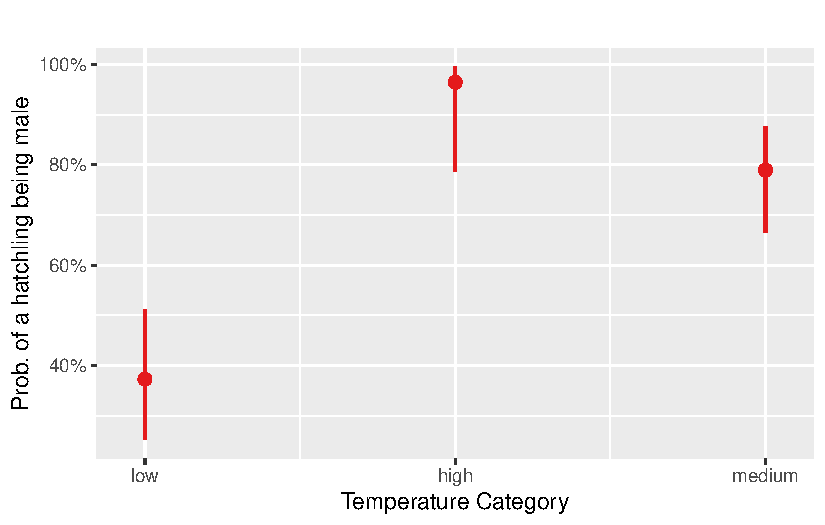
\includegraphics{index_files/figure-pdf/unnamed-chunk-21-1.pdf}

\section{Models for multiple categorical
responses}\label{models-for-multiple-categorical-responses}

Now that we have covered GLMs for categorical responses with two
possible outcomes, we will generalise this to situations where the
response variable is categorical with more than two categories. More
specifically, we will look at logistic regression models applied to
\textbf{nominal} (unordered) responses with \textbf{more than two
categories}.

The basis for modelling categorical data with more than two categories
is the \textbf{multinomial distribution}.

Consider a random variable \(Y\) with \(J\) categories. Let
\(p_1,p_2,\dots, p_J\) be the respective probabilities associated with
each of the \(J\) categories, with \(\sum_j^J p_j = 1\). Suppose there
are \(n\) independent observations which result in \(y_1\) outcomes in
category 1, \(y_2\) outcomes in category 2, and so on. Let
\(\mathbf{y}=(y_1,y_2,\dots,y_J)^\intercal\) with
\(\sum_{j=1}^J y_j = n\). We say that \(\mathbf{y}\) follows a
\textbf{multinomial distribution} with probability mass function
(p.m.f.)

\begin{equation}\phantomsection\label{eq-multinomial}{
f(\mathbf{y} | n)=\frac{n!}{y_1! y_2! \dots y_J!}p_1^{y_1}p_2^{y_2}\dots p_J^{y_J}.
}\end{equation}

\begin{tcolorbox}[enhanced jigsaw, leftrule=.75mm, arc=.35mm, colback=white, opacityback=0, breakable, title=\textcolor{quarto-callout-note-color}{\faInfo}\hspace{0.5em}{Note}, toprule=.15mm, opacitybacktitle=0.6, titlerule=0mm, rightrule=.15mm, bottomtitle=1mm, coltitle=black, toptitle=1mm, colframe=quarto-callout-note-color-frame, bottomrule=.15mm, colbacktitle=quarto-callout-note-color!10!white, left=2mm]

If \(J=2\) then \(p_2=1-p_1\) and \(y_2=n-y_1\) so the expression above
reduces to the p.m.f. of the binomial distribution:

\[
f(\mathbf{y} | n)=\frac{n!}{y_1! (n-y_1)!} p_1^{y_1}p_2^{n-y_1}
\]

\end{tcolorbox}

For the multinomial distribution, we have the following expressions for
the mean, variance and covariance:

\[
\begin{aligned}
\textrm{E}(Y_j)&=np_j\\\textrm{Var}(Y_j)&=np_j(1-p_j)\\\textrm{Cov}(Y_j,Y_k)&= -n p_jp_k
\end{aligned}
\]

Notice also the negative covariance between \(Y_j\) and \(Y_k\) due to
the sum constraint \(\sum_{j=1}^J y_j = n\).

In general, the multinomial model does not satisfy the exponential
family distribution requirement for the response in a GLM, but we can
still fit GLMs to multinomial responses thanks to its relationship with
the Poisson distribution, which is a member of the exponential family.

\begin{tcolorbox}[enhanced jigsaw, leftrule=.75mm, arc=.35mm, colback=white, opacityback=0, breakable, title={Task}, toprule=.15mm, opacitybacktitle=0.6, titlerule=0mm, rightrule=.15mm, bottomtitle=1mm, coltitle=black, toptitle=1mm, colframe=quarto-callout-warning-color-frame, bottomrule=.15mm, colbacktitle=quarto-callout-warning-color!10!white, left=2mm]

Let \(Y_j \sim \text{Po}(\mu_j)\) where the \(Y_j\) are independent for
\(j=1,\dots,J\) with \(\mu_j\) the expected number of events. Their
joint p.m.f. is:
\[ f(\mathbf{y})=\prod_{j=1}^J \frac{\mu_j^{y_j}e^{-\mu_j}}{y_j!}.\]

The random variable \(N=Y_1+Y_2+\dots+Y_J\) follows a
\(\mathrm{Poisson}(\mu_1+\mu_2+\dots+\mu_J)\) density ,
i.e.~\[f(n) = \dfrac{\left(\sum_{j=1}^J\mu_j\right)^ne^{-\sum_{j=1}^J\mu_j}}{n!}.\]

Conditional on \(N\), show that \(\mathbf{y}\) follows a multinomial
distribution.

Take hint

When we condition on the observed total number of events \(N=n\), the
conditional probability
\(f(\mathbf{y}|n) = \dfrac{f(\mathbf{y},n)}{f(n)} = \dfrac{f(y_1,y_2,\ldots,y_n)}{f(n)}\)
since \(N = \sum_{j=1}^J Y_j\). Thus, conditional on \(N=n\),
\(\mathbf{y}\) has the following distribution:

\[
f(\mathbf{y} |n ) =\frac{\prod_{j=1}^J \mu_j^{y_j}e^{-\mu_j}/y_j!}{(\mu_1+\mu_2+\dots+\mu_J)^ne^{-(\mu_1+\mu_2+\dots+\mu_J)}/n!}
\]

See solution

Conditional on \(N=n\), \(\mathbf{y}\) has the following distribution:

\[
f(\mathbf{y} |n ) =\frac{\prod_{j=1}^J \mu_j^{y_j}e^{-\mu_j}/y_j!}{(\mu_1+\mu_2+\dots+\mu_J)^ne^{-(\mu_1+\mu_2+\dots+\mu_J)}/n!}
\]

which can be simplified as:

\[
\begin{aligned}
f(\mathbf{y} |n ) &=\dfrac{\left(\prod_{j=1}^J \frac{\mu_j^{y_j}}{y_j!}\right)\color{red}{e^{-\sum_{j=1}^J \mu_j}}}{ \frac{(\mu_1+\mu_2+\dots+\mu_J)^n\color{red}{e^{-\sum_{j=1}^J \mu_j}}}{n!}} \\&= \dfrac{n!}{y_1!y_2!\ldots y_J!}\dfrac{\prod_{j=1}^J\mu_j^{y_j}}{(\mu_1+\mu_2+\dots+\mu_J)^n}
\end{aligned}
\]

Letting \(n= \sum_{j=1}^J y_j\) and
\(p_j = \dfrac{\mu_j}{\mu_1+\ldots+\mu_J}\), s.t. \(\sum_{j=1}^J p_j=1\)

\[
\begin{aligned}
 f(\mathbf{y}|n)&= \dfrac{n!}{y_1!y_2!\ldots y_J!} \prod_{j=1}^J\left(\dfrac{\mu_j}{\mu_1+\ldots+\mu_J}\right)^{y_j} \\&= \dfrac{n!}{y_1!y_2!\ldots y_J!} \prod_{j=1}^Jp _j^{y_j}
\end{aligned}
\]

which is the same as the expression for the multinomial p.m.f. in
Equation~\ref{eq-multinomial}

\end{tcolorbox}

\subsection{Nominal logistic
regression}\label{nominal-logistic-regression}

Nominal logistic regression, also known as \emph{multinomial logistic
regression} is used when there is no natural order among the response
categories, for example:

\begin{itemize}
\tightlist
\item
  Eye colour: Blue, Green, Brown, Hazel
\item
  House types: Bungalow, Duplex, Terrace
\item
  Type of pet: Dog, Cat, Rodent, Fish, Bird
\item
  Genotype: AA, Aa, aa
\end{itemize}

The goal is to estimate the probabilities for each class \(j\) (where
\(j \in \{1,2,\ldots,J\}\)) based on the independent variables
\(\mathbf{x}\). The probability of the \(j\)th class is then given by:

\[
P(Y=j|\mathbf{x})= \dfrac{\mathrm{exp}(\mathbf{x}^\intercal \boldsymbol{\beta}_j)}{\sum_{k=1}^J\mathrm{exp}(\mathbf{x}^\intercal \boldsymbol{\beta}_k)}
\]

Typically, one category is arbitrarily chosen as the reference category,
and all other categories are compared with it. Suppose category \(J\) is
chosen as the reference category. The \textbf{log-odds} for the other
categories relative to the reference are:

\begin{equation}\phantomsection\label{eq-nominalresp}{
\mathrm{log}\left(\dfrac{P(Y=j|\mathbf{x})}{P(Y=J|\mathbf{x})}\right) = \mathrm{log}\left(\dfrac{p_j}{p_J}\right) =\mathbf{x}^\intercal\boldsymbol{\beta}_j, ~~\text{for } j=1,\dots,J-1.
}\end{equation}

\subsection{Parameter estimation and fitted
values}\label{parameter-estimation-and-fitted-values}

The \(J-1\) log-odds in Equation~\ref{eq-nominalresp} are solved
simultaneously to estimate the parameters \(\boldsymbol{\beta}_j\).

Given parameter estimates \(\hat{\boldsymbol{\beta}}_j\), the linear
predictors \(\mathbf{x}^\intercal\hat{\boldsymbol{\beta}}_j\) can be
calculated.

From Equation~\ref{eq-nominalresp}, we derive:

\begin{equation}\phantomsection\label{eq-pj}{
\hat{p}_j=\hat{p}_J\mathrm{exp}(\mathbf{x}^\intercal\hat{\boldsymbol{\beta}}_j) 
}\end{equation}

Now we can express \(\hat{p}_J\) in terms of the other probabilities by
using the fact that
\(\sum_{j=1}^{J-1} \hat{p}_j + \hat{p}_J = \hat{p}_1+\hat{p}_2+\dots+\hat{p}_J= 1.\)
For instance, substituting Equation~\ref{eq-pj} for \(j = 1,\ldots,J-1\)
in the sumation above yields to:

\[
\sum_{j=1}^{J-1} \hat{p}_J\mathrm{exp}(\mathbf{x}^\intercal\hat{\boldsymbol{\beta}}_j) + \hat{p}_J = 1.
\]

Solving for \(\hat{p}_J\) yields to

\begin{equation}\phantomsection\label{eq-p1hat}{
\hat{p}_J\left(\sum_{j=1}^{J-1} \mathrm{exp}(\mathbf{x}^\intercal\hat{\boldsymbol{\beta}}_j) + 1\right) = 1 \\ \Rightarrow\hat{p}_J = \dfrac{1}{1+\sum_{j=1}^{J-1} \mathrm{exp}(\mathbf{x}^\intercal\hat{\boldsymbol{\beta}}_j)}
}\end{equation}

Hence, the probabilities for each class are:

\begin{itemize}
\item
  For the reference class \(J:\)\[
      \hat{p}_J = \dfrac{1}{1+\sum_{j=1}^{J-1} \mathrm{exp}(\mathbf{x}^\intercal\hat{\boldsymbol{\beta}}_j)}
      \]
\item
  By substituting \(\hat{p}_J\) in Equation~\ref{eq-pj} we find
  \(\hat{p}_j\) for class \(j = 1,2,\ldots,J-1:\)
  \begin{equation}\phantomsection\label{eq-pjhat}{\hat{p}_j=\dfrac{\exp(\mathbf{x}^\intercal\hat{\boldsymbol{\beta}}_j)}{1+\sum_{j=1}^{J-1}\exp(\mathbf{x}^\intercal\hat{\boldsymbol{\beta}}_j)}.}\end{equation}
\end{itemize}

Fitted values (expected frequencies) can be calculated for each
covariate pattern by multiplying the estimated probabilities
\(\hat{p}_j\) by the total frequency of the covariate pattern. Parameter
estimates \(\hat{\boldsymbol{\beta}}_j\) depend on the choice of
reference category, but estimated probabilities and hence, fitted values
(predicted counts), don't.

\subsection{Example: Fitting a nominal logistic regression in
R}\label{example-fitting-a-nominal-logistic-regression-in-r}

In this example we look at data on subjects that were interviewed about
the importance of various features when buying a car (McFadden et al.
2000).

We focus in particular on the importance of power steering and air
conditioning. The variables available in this dataset are:

\begin{itemize}
\tightlist
\item
  \texttt{sex}: woman/man
\item
  \texttt{age}: 18-23, 24-40, \textgreater40
\item
  \texttt{response}: no/little, important, very important
\item
  \texttt{frequency}: number of interviewed people on each group
\end{itemize}

The data set is available on the \texttt{dobson} R package or can be
downloaded below:

Lets begin loading it and produce some exploratory plots.

\begin{Shaded}
\begin{Highlighting}[]
\NormalTok{dcars }\OtherTok{=} \FunctionTok{read.csv}\NormalTok{(}\StringTok{"Cars.csv"}\NormalTok{,}\AttributeTok{stringsAsFactors =}\NormalTok{ T)}

\CommentTok{\# Set "no/little" and "18{-}23"  as our reference categories}

\NormalTok{dcars }\OtherTok{=}\NormalTok{ dcars }\SpecialCharTok{\%\textgreater{}\%}
  \FunctionTok{mutate}\NormalTok{(}\AttributeTok{response =} \FunctionTok{relevel}\NormalTok{(response,}\AttributeTok{ref =} \StringTok{"no/little"}\NormalTok{),}
         \AttributeTok{age =} \FunctionTok{relevel}\NormalTok{(age,}\AttributeTok{ref=}\StringTok{"18{-}23"}\NormalTok{)) }
\end{Highlighting}
\end{Shaded}

\begin{longtable}[]{@{}lllr@{}}
\toprule\noalign{}
sex & age & response & frequency \\
\midrule\noalign{}
\endhead
\bottomrule\noalign{}
\endlastfoot
women & 18-23 & no/little & 26 \\
women & 18-23 & important & 12 \\
women & 18-23 & very important & 7 \\
women & 24-40 & no/little & 9 \\
women & 24-40 & important & 21 \\
women & 24-40 & very important & 15 \\
women & \textgreater{} 40 & no/little & 5 \\
women & \textgreater{} 40 & important & 14 \\
women & \textgreater{} 40 & very important & 41 \\
men & 18-23 & no/little & 40 \\
men & 18-23 & important & 17 \\
men & 18-23 & very important & 8 \\
men & 24-40 & no/little & 17 \\
men & 24-40 & important & 15 \\
men & 24-40 & very important & 12 \\
men & \textgreater{} 40 & no/little & 8 \\
men & \textgreater{} 40 & important & 15 \\
men & \textgreater{} 40 & very important & 18 \\
\end{longtable}

From the plots of the data below, we can see that quite a large
proportion of people -- a little over 58\% in the over 40 category
considered the features \emph{very important} and, similarly 60\% of
young people (18-23 years old) considered these features as having
\emph{no or little importance}. Sex also seems to have an impact on car
feature preferences, with over 40\% of men considering the features of
\emph{no or little importance} and over 40\% of women considering them
\emph{very important}.

\subsection{R Plot}

\begin{figure}[H]

{\centering 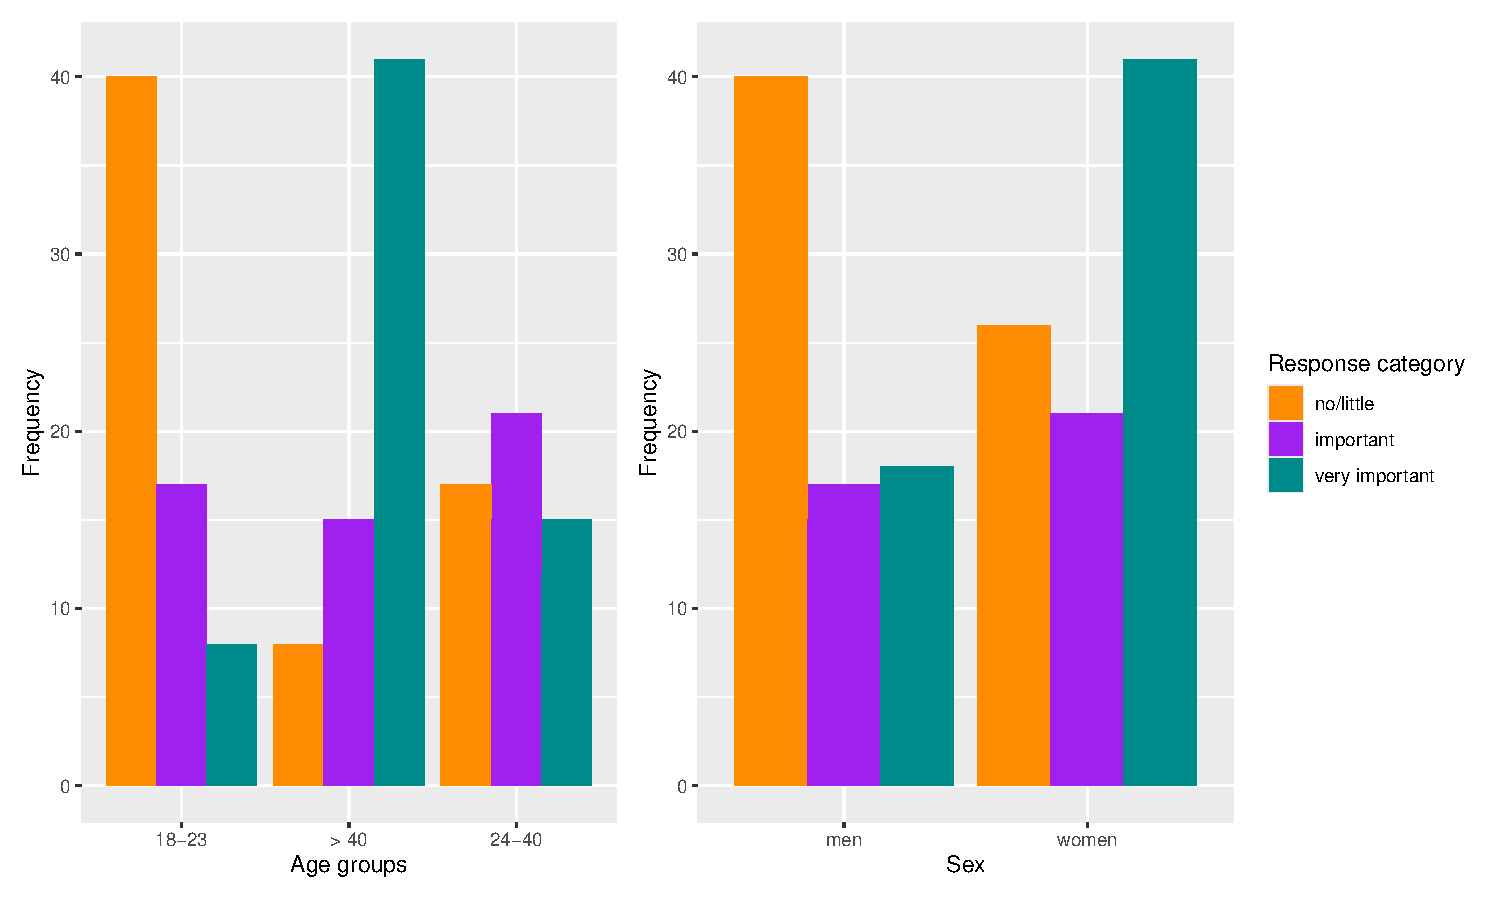
\includegraphics{index_files/figure-pdf/unnamed-chunk-24-1.pdf}

}

\caption{Preferences for air conditioning and power steering in cars by
gender and age.}

\end{figure}%

\subsection{R Code}

\begin{Shaded}
\begin{Highlighting}[]
 \FunctionTok{ggplot}\NormalTok{(dcars, }\FunctionTok{aes}\NormalTok{(}\AttributeTok{x =}\NormalTok{ age,}
                   \AttributeTok{y =}\NormalTok{ frequency, }
                   \AttributeTok{fill =}\NormalTok{ response)) }\SpecialCharTok{+}
      \FunctionTok{geom\_bar}\NormalTok{(}\AttributeTok{stat =} \StringTok{"identity"}\NormalTok{,}
               \AttributeTok{position =} \StringTok{"dodge"}\NormalTok{ )}\SpecialCharTok{+}
   \FunctionTok{labs}\NormalTok{(}\AttributeTok{x =} \StringTok{"Age groups"}\NormalTok{,}\AttributeTok{y =}\StringTok{"Frequency"}\NormalTok{)}\SpecialCharTok{+}
   \FunctionTok{scale\_fill\_manual}\NormalTok{(}\AttributeTok{name =} \StringTok{"Response category"}\NormalTok{,}
                     \AttributeTok{values =} \FunctionTok{c}\NormalTok{(}\StringTok{"darkorange"}\NormalTok{,}\StringTok{"purple"}\NormalTok{,}\StringTok{"cyan4"}\NormalTok{)) }
\end{Highlighting}
\end{Shaded}

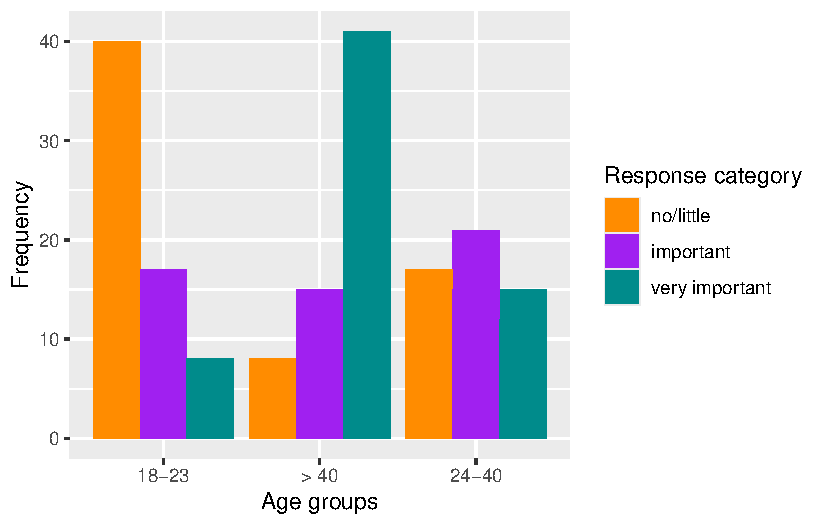
\includegraphics{index_files/figure-pdf/unnamed-chunk-25-1.pdf}

\begin{Shaded}
\begin{Highlighting}[]
 \FunctionTok{ggplot}\NormalTok{(dcars, }\FunctionTok{aes}\NormalTok{(}\AttributeTok{x =}\NormalTok{ sex,}
                   \AttributeTok{y =}\NormalTok{ frequency, }
                   \AttributeTok{fill =}\NormalTok{ response)) }\SpecialCharTok{+}
      \FunctionTok{geom\_bar}\NormalTok{(}\AttributeTok{stat =} \StringTok{"identity"}\NormalTok{,}
               \AttributeTok{position =} \StringTok{"dodge"}\NormalTok{ )}\SpecialCharTok{+}
   \FunctionTok{labs}\NormalTok{(}\AttributeTok{x =} \StringTok{"Sex"}\NormalTok{,}\AttributeTok{y =}\StringTok{"Frequency"}\NormalTok{)}\SpecialCharTok{+}
      \FunctionTok{scale\_fill\_manual}\NormalTok{(}\AttributeTok{name =} \StringTok{"Response category"}\NormalTok{,}
                        \AttributeTok{values =} \FunctionTok{c}\NormalTok{(}\StringTok{"darkorange"}\NormalTok{,}\StringTok{"purple"}\NormalTok{,}\StringTok{"cyan4"}\NormalTok{)) }
\end{Highlighting}
\end{Shaded}

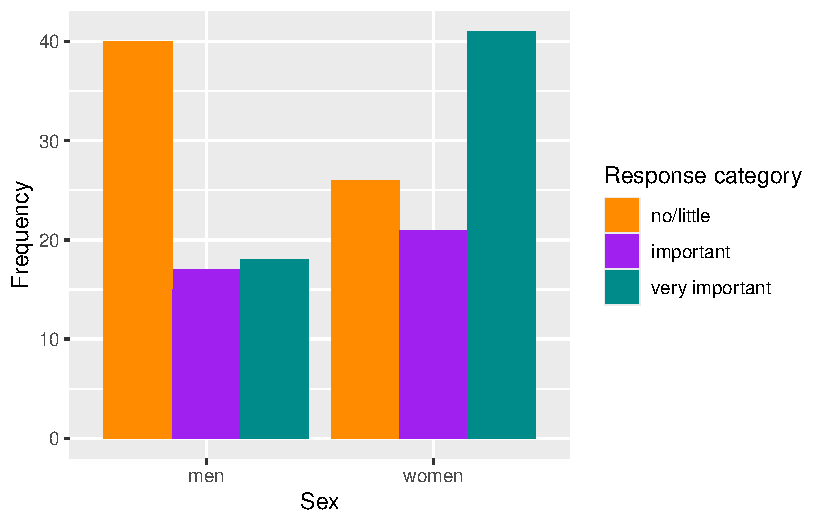
\includegraphics{index_files/figure-pdf/unnamed-chunk-25-2.pdf}

Although the response is really an ordinal variable, we will treat it as
nominal with ``no/little importance'' as the reference category (also
occasionally referred to as ``unimportant'' in the rest for brevity.).
Similarly we will initially regard \texttt{age} as nominal.

We can fit the following \textbf{nominal logistic regression model}
using the \texttt{multinom()} function from \texttt{library(nnet)}:

\begin{equation}\phantomsection\label{eq-multi_mod}{
\mathrm{log}\left(\frac{p_j}{p_1} \right) = \beta_{0j}+\beta_{1j}x_1+\beta_{2j}x_2+\beta_{3j}x_3, ~~ j=2,3
}\end{equation}

where

\begin{itemize}
\tightlist
\item
  \(j=1\) for ``no/little importance'' (the reference category)
\item
  \(j=2\) for ``important''
\item
  \(j=3\) for ``very important''
\item
  \(x_1=1\) for women and 0 for men,
\item
  \(x_2=1\) for age 24-40 years and 0 otherwise
\item
  \(x_3=1\) for age \(>\) 40 years and 0 otherwise.
\end{itemize}

\begin{Shaded}
\begin{Highlighting}[]
\FunctionTok{library}\NormalTok{(nnet)}
\NormalTok{model\_cars }\OtherTok{\textless{}{-}} \FunctionTok{multinom}\NormalTok{(response }\SpecialCharTok{\textasciitilde{}}\NormalTok{ age }\SpecialCharTok{+}\NormalTok{ sex, }\AttributeTok{weight =}\NormalTok{ frequency, }\AttributeTok{data =}\NormalTok{ dcars)}
\end{Highlighting}
\end{Shaded}

\begin{verbatim}
# weights:  15 (8 variable)
initial  value 329.583687 
iter  10 value 290.566455
final  value 290.351098 
converged
\end{verbatim}

Notice that model converged after 10 iterations, the default number of
iteration is set to 100 but you can modify this by setting
\texttt{maxit=X} where \texttt{X} is the number of iterations after
which the algorithm will stop.

Let look at model summaries and interpret the coefficients.

\begin{Shaded}
\begin{Highlighting}[]
\NormalTok{model\_cars }\SpecialCharTok{\%\textgreater{}\%} \FunctionTok{tab\_model}\NormalTok{(}\AttributeTok{transform =} \ConstantTok{NULL}\NormalTok{)}
\end{Highlighting}
\end{Shaded}

\begin{longtable}[]{@{}ccccc@{}}
\toprule\noalign{}
\endhead
\bottomrule\noalign{}
\endlastfoot
~ & \multicolumn{4}{c@{}}{%
response} \\
Predictors & Log-Odds & CI & p & Response \\
(Intercept) & -0.98 & -1.55~--~-0.41 & \textbf{0.003} & important \\
age {[}\textgreater{} 40{]} & 1.59 & 0.69~--~2.49 & \textbf{0.003} &
important \\
age24-40 & 1.13 & 0.37~--~1.89 & \textbf{0.008} & important \\
sex {[}women{]} & 0.39 & -0.28~--~1.06 & 0.226 & important \\
(Intercept) & -1.85 & -2.59~--~-1.12 & \textbf{\textless0.001} & very
important \\
age {[}\textgreater{} 40{]} & 2.92 & 1.97~--~3.86 &
\textbf{\textless0.001} & very important \\
age24-40 & 1.48 & 0.58~--~2.37 & \textbf{0.004} & very important \\
sex {[}women{]} & 0.81 & 0.10~--~1.53 & \textbf{0.030} & very
important \\
Observations & \multicolumn{4}{l@{}}{%
18} \\
R\textsuperscript{2} / R\textsuperscript{2} adjusted &
\multicolumn{4}{l@{}}{%
0.118 / 0.115} \\
\end{longtable}

Notice the two sets of coefficients, for the \texttt{response\ column}
categories \texttt{important} and \texttt{very\ important} that
correspond to the two log-odds equations comparing these to the
baseline, which is \texttt{no/little\ importance}.

Lets break this down:

\begin{itemize}
\item
  First, \(\hat{\beta}_{0,\text{important}} = -0.98\) represent the
  \textbf{log-odds} of considering the features \texttt{important} vs
  \texttt{no/little} important for \texttt{men} between \texttt{18-23}
  since these are our two reference categories ( this is the case when
  \(x_{1} = x_2 = x_3 = 0\) in Equation~\ref{eq-multi_mod}).
\item
  Likewise, \(\hat{\beta}_{0,\text{very important}} = -1.85\) represent
  the \textbf{log-odds} of considering the features
  \texttt{very\ important} vs \texttt{no/little} important for
  \texttt{men} between \texttt{18-23}.
\item
  Then, each \(\hat{\beta}_{i,j}\) shows how the log-odds change when
  moving from the reference categories to the other levels. For example,
  the \textbf{log-odds} of considering the feature \texttt{important} vs
  \texttt{no/little\ important} for \texttt{women} between
  \texttt{24-40} are given by :
\end{itemize}

\[
\begin{aligned}
\mathrm{log}\left(\frac{p_{(\text{important|age>40,sex=women})}}{p_{(\text{no/little|age > 40,sex=women})}} \right) &= \hat{\beta}_{0,\text{important}}+\hat{\beta}_{1,\text{important}} x_1 +\hat{\beta}_{2\text{important}}x_2\\
&= -0.98 +  0.39 + 1.13  \approx 0.54
\end{aligned}
\]

However, it might be easier to interpret these coefficients in terms of
odds for each logit equation. For example:

\begin{Shaded}
\begin{Highlighting}[]
\NormalTok{model\_cars }\SpecialCharTok{\%\textgreater{}\%} \FunctionTok{tab\_model}\NormalTok{(}\AttributeTok{transform =} \StringTok{"exp"}\NormalTok{)}
\end{Highlighting}
\end{Shaded}

From this table, we can see that the odds of considering the features
important (versus \texttt{no/little\ importance}) for a person of the
same gender over 40 years are \textbf{4.89} times the odds for 18-23
year old person (which is the baseline category for the \texttt{age}
group). Remember that this is calculated based on the
\textbf{odds-ratio} as follows:

\[
\begin{aligned}
\dfrac{\text{Odds}(\text{important|age > 40 })}{\text{Odds}(\text{important|age [18-23] })} &= \dfrac{\exp(\cancel{\hat{\beta}_{\text{0,important}}} + \cancel{\hat{\beta}_{\text{1,important}}} x_1 + \hat{\beta}_{\text{2,important}} \cancelto{0}{x_2}+ \hat{\beta}_{3,\text{important}} x_3 )}{\exp(\cancel{\hat{\beta}_{\text{0,important}}} + \cancel{\hat{\beta}_{\text{1,important}}} x_1)}\\
&= \exp(\hat{\beta}_{3,\text{important}} ) = 4.89
\end{aligned}
\]

In general, a positive coefficient (or greater than 1 odds multiplier)
tells us that older people are more likely to consider the features
important than young people, which is consistent with what we observed
in the exploratory plots. Similarly, we can see that women are more
likely than men to consider the features important, specifically the
chances a woman finds these features \texttt{important} are 47\% greater
than men and more than twice consider these features as
\texttt{very\ important} compared to men:

\[
\begin{aligned} \dfrac{\text{Odds}(\text{important|sex = women })}{\text{Odds}(\text{important|sex= men })} &= \dfrac{\exp(\cancel{\hat{\beta}_{\text{0,important}}} + \hat{\beta}_{\text{1,important}} x_1 + \cancel{\hat{\beta}_{\text{2,important}}} x_2+ \cancel{\hat{\beta}_{3,\text{important}}} x_3 )}{\exp(\cancel{\hat{\beta}_{\text{0,important}}} + \hat{\beta}_{\text{1,important}} \cancelto{0}{x_1} + \cancel{\hat{\beta}_{\text{2,important}}} x_2 + \cancel{\hat{\beta}_{3,\text{important}}} x_3)}\\
&= \exp(\hat{\beta}_{1,\text{important}}) = 1.47 
\end{aligned}
\]

\[ 
\begin{aligned} 
\dfrac{\text{Odds}(\text{very important|sex = women })}{\text{Odds}(\text{very important|sex= men })} &= \dfrac{\exp(\cancel{\hat{\beta}_{\text{0, very very important}}} + \hat{\beta}_{\text{1, very important}} x_1 + \cancel{\hat{\beta}_{\text{2,very important}}} x_2+ \cancel{\hat{\beta}_{3,\text{ very important}}} x_3 )}{\exp(\cancel{\hat{\beta}_{\text{0,very important}}} + \hat{\beta}_{\text{1,very important}} \cancelto{0}{x_1} + \cancel{\hat{\beta}_{\text{2,important}}} x_2 + \cancel{\hat{\beta}_{3,\text{important}}} x_3)}\\
&= \exp(\hat{\beta}_{1,\text{very important}}) = 2.25 
\end{aligned} 
\]

However, in the first case, the difference between women and men is not
statistically significant since the 95\% CI contains 1.

\subsection{Model checking and model
comparisons}\label{model-checking-and-model-comparisons}

Summary statistics can be used to assess the adequacy of a model and
also to compare models. Some of the statistics we can consider are:

\begin{itemize}
\tightlist
\item
  the \textbf{deviance}
  \(D=2[l(\hat{\boldsymbol{\beta}}_{\max})-l(\hat{\boldsymbol{\beta}})]\)
  (also referred to as \emph{residual deviance}), where
  \(l(\hat{\boldsymbol{\beta}}_{\max})\) is the maximised log-likelihood
  for the saturated (full) model and \(l(\hat{\boldsymbol{\beta}})\) is
  the maximised log-likelihood for the model of interest;
\item
  the \textbf{likelihood ratio statistic}, which is equal to the
  difference between the null deviance (deviance of the model with no
  predictors included) and the residual deviance for the model of
  interest;
\item
  the \textbf{Akaike information criterion}
  \(AIC=-2l(\hat{\boldsymbol{\beta}};\mathbf{y})+2p\), which equals the
  maximised log-likelihood of the model of interest plus a penalty term
  equal to twice the number of parameters in the model. The reason for
  this is that we can keep adding predictors to the model to improve the
  log-likelihood, but the cost is increased model complexity. The
  penalty term attempts to strike a balance between model complexity and
  how well the model fits.
\end{itemize}

If the model fits well, the deviance will be asymptotically
\(\chi^2(N-p)\), where \(N\) is \(J-1\) times the number of distinct
covariate patterns in the data, and \(p\) is the number of parameters
estimated.

The likelihood ratio statistic will be asymptotically
\(\chi^2[p-(J-1)]\) because the null (minimal) model will have one
parameter for each logit defined in Equation~\ref{eq-nominalresp}.

The AIC can be used for model selection: calculate the criterion for
each model and choose the one with the smallest value of the AIC.

We can compare the nominal logistic regression model with additive terms
for \texttt{age} and \texttt{sex} with the null model by taking the
difference in deviances (likelihood ratio test).

The null model can be fit as follows:

\begin{Shaded}
\begin{Highlighting}[]
\NormalTok{model\_null}\OtherTok{\textless{}{-}} \FunctionTok{multinom}\NormalTok{(response }\SpecialCharTok{\textasciitilde{}} \DecValTok{1}\NormalTok{, }\AttributeTok{data=}\NormalTok{dcars, }\AttributeTok{weights=}\NormalTok{frequency)}
\end{Highlighting}
\end{Shaded}

\begin{verbatim}
# weights:  6 (2 variable)
initial  value 329.583687 
final  value 329.272024 
converged
\end{verbatim}

To see some model comparison metrics we can use the \texttt{glance()}
function from the \texttt{broom} package:

\begin{Shaded}
\begin{Highlighting}[]
\FunctionTok{glance}\NormalTok{(model\_null)}
\end{Highlighting}
\end{Shaded}

\begin{verbatim}
# A tibble: 1 x 4
    edf deviance   AIC  nobs
  <dbl>    <dbl> <dbl> <int>
1     2     659.  663.    18
\end{verbatim}

\begin{Shaded}
\begin{Highlighting}[]
\FunctionTok{glance}\NormalTok{(model\_cars)}
\end{Highlighting}
\end{Shaded}

\begin{verbatim}
# A tibble: 1 x 4
    edf deviance   AIC  nobs
  <dbl>    <dbl> <dbl> <int>
1     8     581.  597.    18
\end{verbatim}

The difference in deviance is \(658.54-580.70=77.84\) which is
significant when compared with a \(\chi^2(8-2)\):

\begin{Shaded}
\begin{Highlighting}[]
\FunctionTok{qchisq}\NormalTok{(}\AttributeTok{df=}\DecValTok{6}\NormalTok{, }\AttributeTok{p=}\FloatTok{0.95}\NormalTok{)}
\end{Highlighting}
\end{Shaded}

\begin{verbatim}
[1] 12.59159
\end{verbatim}

\begin{Shaded}
\begin{Highlighting}[]
\CommentTok{\# pval}
\FunctionTok{pchisq}\NormalTok{(}\FloatTok{77.844}\NormalTok{,}\AttributeTok{df=}\DecValTok{6}\NormalTok{,}\AttributeTok{lower.tail =}\NormalTok{ F)}
\end{Highlighting}
\end{Shaded}

\begin{verbatim}
[1] 9.955365e-15
\end{verbatim}

Alternatively, we can run the likelihood ratio test using the anova
function as follows:

\begin{Shaded}
\begin{Highlighting}[]
\FunctionTok{anova}\NormalTok{(model\_null,model\_cars,}\AttributeTok{test =} \StringTok{"Chisq"}\NormalTok{)}
\end{Highlighting}
\end{Shaded}

\begin{verbatim}
Likelihood ratio tests of Multinomial Models

Response: response
      Model Resid. df Resid. Dev   Test    Df LR stat.      Pr(Chi)
1         1        34   658.5440                                   
2 age + sex        28   580.7022 1 vs 2     6 77.84185 9.992007e-15
\end{verbatim}

Overall, the explanatory variables are descriptive of car preferences.

We can also compare this model with the saturated (full) model, which
includes an interaction between \texttt{age} and \texttt{sex}:

\begin{Shaded}
\begin{Highlighting}[]
\NormalTok{model\_full }\OtherTok{\textless{}{-}} \FunctionTok{multinom}\NormalTok{(response }\SpecialCharTok{\textasciitilde{}}\NormalTok{ age }\SpecialCharTok{*}\NormalTok{ sex, }\AttributeTok{weight =}\NormalTok{ frequency, }\AttributeTok{data =}\NormalTok{ dcars)}
\end{Highlighting}
\end{Shaded}

\begin{verbatim}
# weights:  21 (12 variable)
initial  value 329.583687 
iter  10 value 288.541004
final  value 288.381742 
converged
\end{verbatim}

\begin{Shaded}
\begin{Highlighting}[]
\FunctionTok{glance}\NormalTok{(model\_full)}
\end{Highlighting}
\end{Shaded}

\begin{verbatim}
# A tibble: 1 x 4
    edf deviance   AIC  nobs
  <dbl>    <dbl> <dbl> <int>
1    12     577.  601.    18
\end{verbatim}

The difference in deviance between the additive and the saturated model
is \(580.70-576.76=3.94\). This is not significant when compared with a
\(\chi^2(12-8)\), so the additive model appears to fit the data well.

\begin{Shaded}
\begin{Highlighting}[]
\FunctionTok{qchisq}\NormalTok{(}\AttributeTok{df=}\DecValTok{4}\NormalTok{, }\AttributeTok{p=}\FloatTok{0.95}\NormalTok{)}
\end{Highlighting}
\end{Shaded}

\begin{verbatim}
[1] 9.487729
\end{verbatim}

\begin{Shaded}
\begin{Highlighting}[]
\CommentTok{\# pval}
\FunctionTok{pchisq}\NormalTok{(}\FloatTok{3.94}\NormalTok{,}\AttributeTok{df=}\DecValTok{4}\NormalTok{,}\AttributeTok{lower.tail =}\NormalTok{ F)}
\end{Highlighting}
\end{Shaded}

\begin{verbatim}
[1] 0.4141869
\end{verbatim}

Again, we can use the \texttt{anova} function to compare the three
nested models:

\begin{Shaded}
\begin{Highlighting}[]
\FunctionTok{anova}\NormalTok{(model\_null,model\_cars,model\_full,}\AttributeTok{test =} \StringTok{"Chisq"}\NormalTok{) }
\end{Highlighting}
\end{Shaded}

\begin{verbatim}
Likelihood ratio tests of Multinomial Models

Response: response
      Model Resid. df Resid. Dev   Test    Df  LR stat.      Pr(Chi)
1         1        34   658.5440                                    
2 age + sex        28   580.7022 1 vs 2     6 77.841851 9.992007e-15
3 age * sex        24   576.7635 2 vs 3     4  3.938713 4.143637e-01
\end{verbatim}

The same conclusion is supported when comparing the AIC for these
models:

\begin{Shaded}
\begin{Highlighting}[]
\FunctionTok{library}\NormalTok{(performance)}
\FunctionTok{compare\_performance}\NormalTok{(model\_full,model\_cars,model\_null,}\AttributeTok{metrics =} \StringTok{"AIC"}\NormalTok{)}
\end{Highlighting}
\end{Shaded}

\begin{longtable}[]{@{}llrr@{}}
\toprule\noalign{}
Name & Model & AIC & AIC\_wt \\
\midrule\noalign{}
\endhead
\bottomrule\noalign{}
\endlastfoot
model\_full & multinom & 600.76 & 0.12 \\
model\_cars & multinom & 596.70 & 0.88 \\
model\_null & multinom & 662.54 & 0.00 \\
\end{longtable}

the additive model has a smaller AIC of 596.7 compared to the
interaction model which has AIC of 600.7.

\begin{tcolorbox}[enhanced jigsaw, leftrule=.75mm, arc=.35mm, colback=white, opacityback=0, breakable, title={Task}, toprule=.15mm, opacitybacktitle=0.6, titlerule=0mm, rightrule=.15mm, bottomtitle=1mm, coltitle=black, toptitle=1mm, colframe=quarto-callout-warning-color-frame, bottomrule=.15mm, colbacktitle=quarto-callout-warning-color!10!white, left=2mm]

The \texttt{iris} data set gives the measurements in centimeters of the
variables sepal length and width and petal length and width,
respectively, for 50 flowers from each of three species of iris: setosa,
versicolor, and virginica. Suppose that we have these measurements from
an iris and we wish to classify it into one of the three species.

Fit a nominal logistic regression model to the data and predict the
probability of each species from the fitted model using sepal length as
the only predictor.

Note that you can use the predicted probabilities from a nominal
logistic regression model to classify an observation to the category
with the highest predicted probability.

Take hint

We can get a list which assigns each observation to the category with
the highest predicted probability using \texttt{predict(your\_model)}.

See solution

\begin{Shaded}
\begin{Highlighting}[]
\NormalTok{m.iris }\OtherTok{\textless{}{-}} \FunctionTok{multinom}\NormalTok{(Species }\SpecialCharTok{\textasciitilde{}}\NormalTok{ Sepal.Length, }\AttributeTok{data=}\NormalTok{iris)}
\end{Highlighting}
\end{Shaded}

\begin{verbatim}
# weights:  9 (4 variable)
initial  value 164.791843 
iter  10 value 91.337114
iter  20 value 91.035008
final  value 91.033971 
converged
\end{verbatim}

\begin{Shaded}
\begin{Highlighting}[]
\FunctionTok{cbind}\NormalTok{(iris,}\FunctionTok{predict}\NormalTok{(m.iris)) }\SpecialCharTok{\%\textgreater{}\%} \FunctionTok{head}\NormalTok{()}
\end{Highlighting}
\end{Shaded}

\begin{verbatim}
  Sepal.Length Sepal.Width Petal.Length Petal.Width Species predict(m.iris)
1          5.1         3.5          1.4         0.2  setosa          setosa
2          4.9         3.0          1.4         0.2  setosa          setosa
3          4.7         3.2          1.3         0.2  setosa          setosa
4          4.6         3.1          1.5         0.2  setosa          setosa
5          5.0         3.6          1.4         0.2  setosa          setosa
6          5.4         3.9          1.7         0.4  setosa          setosa
\end{verbatim}

\end{tcolorbox}

In the car preferences example there was a natural ordering among the
response categories that we have not accounted for. This ordering can be
taken into account in the model specification. Unfortunately, we don't
have time to cover all of this in a single session. But please have a
look at the extra material where we introduce the basis of
\textbf{ordinal logistic regression} for ordered categorical responses.

\phantomsection\label{refs}
\begin{CSLReferences}{1}{0}
\bibitem[\citeproctext]{ref-gelman2006}
Gelman, Andrew, and Jennifer Hill. 2006. {``Data Analysis Using
Regression and Multilevel/Hierarchical Models,''} December.
\url{https://doi.org/10.1017/cbo9780511790942}.

\bibitem[\citeproctext]{ref-mcfadden2000}
McFadden, Michael, Jennifer Powers, Wendy Brown, and Michelle Walker.
2000. {``Vehicle and Driver Attributes Affecting Distance from the
Steering Wheel in Motor Vehicles.''} \emph{Human Factors: The Journal of
the Human Factors and Ergonomics Society} 42 (4): 676--82.
\url{https://doi.org/10.1518/001872000779697971}.

\end{CSLReferences}



\end{document}
